\documentclass[12pt]{ctexart}
\usepackage{geometry}       % 设置页面整体布局
\geometry{top=2.5cm, bottom=2.5cm, left=2cm, right=2cm}
\usepackage{fancyhdr}       % 设置页眉页脚布局
\pagestyle{fancy}
\rhead{\thepage}            % 设置右页眉为页数
\chead{中国科学技术大学}
\cfoot{}                    % 设置中间页脚为空
\usepackage{amsmath}        % 数学公式宏包
\numberwithin{equation}{section}
\usepackage{esint}          % 交叉引用宏包
\usepackage[colorlinks,     % 设置引用的颜色
            linkcolor=black,
            anchorcolor=black,
            urlcolor=cyan,
            citecolor=black,
           ]{hyperref}
\usepackage{makecell}       % 插入表格宏包
\usepackage{longtable}      % 长表格宏包
\usepackage{appendix}       % 生成附录宏包
\usepackage{graphicx}       % 插入图片宏包
\usepackage{epstopdf}       % 插入eps图片宏包
\usepackage{cite}           % 文献引用宏包
\renewcommand{\thefigure}   % 设置图片编号格式
    {\thesection{}.\arabic{figure}}
\renewcommand{\thefootnote}{} % 设置角标编号不出现在文中
                            % 以\footnotetext{Footnotetext without footnote mark}使用
\usepackage{unicode-math}
\usepackage{listings}
\usepackage{hyperref}



\CTEXsetup[format={\Large\bfseries}]{section}


\begin{document}

\nocite{*}

\begin{center}
    \heiti \fontsize{24pt}{0}{稀溶液粘度法测定聚合物的分子量}

    \vspace{12pt}

    \kaishu \fontsize{13.75pt}{0}禤科材

    \footnotetext{\textbf{实验日期:}2022年10月28日}
    \footnotetext{\textbf{作者简介:}禤科材(2002-),男,学号PB20030874,中国科学技术大学本科在读,专业方向为化学物理}
    \footnotetext{\textbf{联系方式:}电话 18108064415 ,邮箱 \href{mailto:ustcxkc@mail.ustc.edu.cn}{ustcxkc@mail.ustc.edu.cn}}

    \vspace{5pt}

    \songti \fontsize{12pt}{0}(中国科学技术大学化学与材料科学学院,安徽 合肥 230026)
\end{center}

\noindent\textbf{摘~~~\!要}~~~\!
高分子物质常常是由不同聚合度的分子组成的混合物,其平均分子量需要
通过一些实验手段测定才能得到。本实验使用乌式黏度计,通过测量聚乙二醇
(20000)的特性黏数,利用经验公式得出了聚乙二醇(20000)的粘均
分子量。此方法具有适用范围广,操作简便等优点。实验同时研究了不同
数据处理方法对该实验结果的影响。
\newline
\textbf{关键字}~~~\!
稀溶液粘度法;聚乙二醇;粘均分子量

\begin{center}
    {\LARGE\rmfamily\textbf{Determination of Molecular Weight of Polymer by Dilute Solution Viscosity Method}}

    \vspace{12pt}

    {\slshape Xuan Kecai}

    \vspace{5pt}

    (School of Chemistry and Material Science, USTC, Hefei 230026, China)
\end{center}

\noindent\textbf{Abstract}~~~\!
Polymer materials are often mixtures of molecules with
different degrees of polymerization, and their average
molecular weight can be obtained only by some experimental
means. In this experiment, the Ukrainian viscometer was used
to measure the intrinsic viscosity of polyethylene glycol
(20000), and the average molecular weight of polyethylene
glycol (20000) was obtained by empirical formula. This method
has the advantages of its wide application and simple
operation. The effects of different data processing methods
on the experimental results were also studied.
\newline
\textbf{Keywords}~~~\!
dilute solution viscosity method, polyethylene glycol,
average viscosity molecular weight

\section{序言}

聚合物是由有机小分子单体聚合而成的高分子物质,由于聚合度$n$的不同,
聚合物的相对分子质量并不是一个确定的值,在实际测量中测量的是其
统计平均分子量。由于统计方法的不同,一种高聚物可有多种平均分子量,
而每一种方法都有它的优缺点和适用的分子量范围$^{[1]}$。本实验采用稀溶液
粘度法测定聚乙二醇的分子量为粘均分子量。由于溶液的粘度与浓度有关,
通过测量不同浓度溶液的相对粘度 $η_r$可以作图外推得到高分子的特性粘数
$[η]$,从而得到高分子溶质的平均相对分子质量,这种方法简单且操作
便利,适用的分子量范围大,又有相当好的实验精确度,是一种目前广泛
应用的测定聚合物分子量的方法。

\section{实验}
\subsection{试剂与仪器}

聚乙二醇20000(国药集团化学试剂有限公司,GR)、蒸馏水。

HK-2A 型超级恒温水水浴(南京南大万和科技有限公司)、HK-1D 型恒温
水槽(南京南大万和科技有限公司)、CPA2245 型分析天平(Sartorius)、
乌氏粘度计(毛细管内径0.55mm)、秒表、10mL和5mL 移液管、50mL
容量瓶、150mL 烧杯、2\# 或3\# 熔砂漏斗、锥形瓶、秒表、注射器、
洗耳球、铅垂线、长尾夹、乳胶管。

\subsection{实验方法}
\subsubsection{高分子溶液的配制}

准确称量0.9000g 的聚乙二醇,溶解,在50mL 容量瓶中定容后转移到
锥形瓶中并密封。将聚乙二醇溶液和用熔砂漏斗过滤过的无尘水放在
30.00$^\circ$C 中保温。

\subsubsection{溶液流出时间的测定}

将乌氏粘度计放在30.00$^\circ$C 的恒温水槽中保温,保持粘度计竖直,在粘度计
B 管和 C 管上套上乳胶管并用长尾夹夹住 C 管乳胶管,向 A 管中准确
移取 10.00 mL 聚乙二醇溶液,用注射器抽取 B 管中的空气使液面上升
至 B 管上方缓冲泡中,同时打开长尾夹使体系与大气连通,测量液体缓慢
流下经过两条刻度线的时间,平行测量 3 次,取平均值。分批准确移取
5.00 mL、5.00 mL、10.00 mL、10.00 mL 无尘水从 A 管注入乌氏粘度计
稀释聚乙二醇至原来浓度的 2/3、1/2、1/3、1/4,混合均匀,再用相同的
方法分别测量各组的时间。

\subsubsection{纯溶剂流出时间的测定}

将粘度计中的溶液倒出,用无尘水洗涤粘度计数遍,按照 2.2.2 的方法测定纯溶剂的流出时间。

\section{结果与讨论}
\subsection{实验结果}
\subsubsection{实验法测定纯溶剂流出时间的实验结果}

实验数据计算结果如下表所示。
\begin{longtable}{ccccccc}
    \caption{实验数据计算结果} \\
    \hline
    溶剂量/mL & 相对浓度$C'$ & 平均流出时间$t$/s & 相对粘度$\eta_\text{r}$ & 特性粘度$\eta_{\text{sp}}$ & $\eta_\text{sp}/C'$ & $\ln\eta_\text{r}/C'$ \\
    \hline
    $0$  & $ 1 $ & $3'36''37$ & $1.8836$ & $0.8836$ & $0.8836$ & $0.6332$ \\
    $5$  & $2/3$ & $3'03''19$ & $1.5941$ & $0.5941$ & $0.8912$ & $0.6995$ \\
    $5$  & $1/2$ & $2'43''59$ & $1.4259$ & $0.4259$ & $0.8518$ & $0.7096$ \\
    $10$ & $1/3$ & $2'25''42$ & $1.2670$ & $0.2670$ & $0.8010$ & $0.7100$ \\
    $10$ & $1/4$ & $2'17''09$ & $1.1926$ & $0.1926$ & $0.7704$ & $0.7045$ \\
    纯溶剂 & $0$ & $1'55''00$ & $1.0000$ & $0.0000$ & / & / \\
    \hline
\end{longtable}

拟合图像如图 3.1 所示。
\begin{figure}[!h]
    \centering
    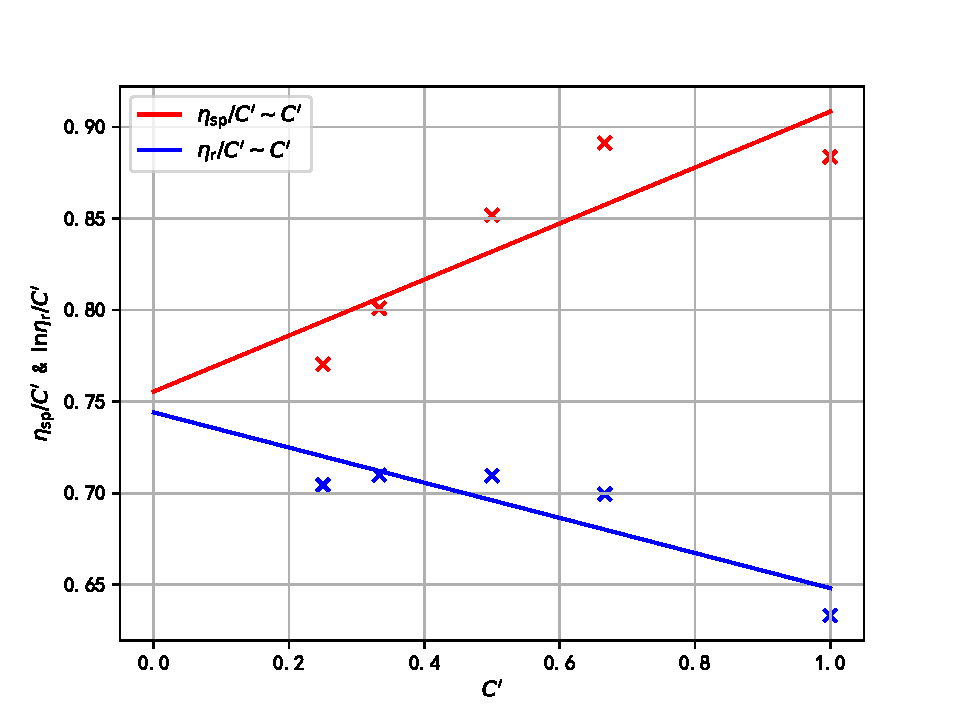
\includegraphics[scale=0.8]{fitting1.pdf}
    \caption{直接作图法拟合曲线}
\end{figure}

拟合方程为
\begin{align}
    \frac{\eta_\text{sp}}{C'} &= 0.1528 C' + 0.7555, \\
    \frac{\ln\eta_\text{sp}}{C'} &= -0.09595 C' + 0.7441.
\end{align}

计算可得$[\eta] = 41.66$mL/g;粘均分子量为
$3.284\times 10^{4}~\mathrm{g/mol}$。

\subsubsection{外推法测定纯溶剂流出时间的实验结果}

由实验数据作出$t\sim C'$图像如图 3.2 所示。
\begin{figure}[!h]
    \centering
    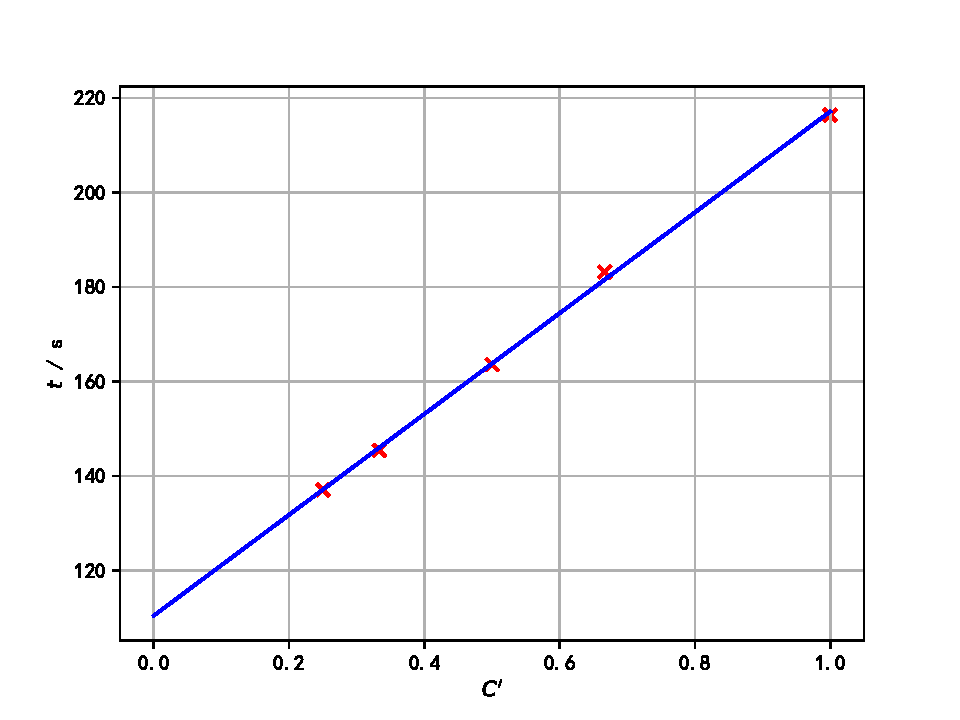
\includegraphics[scale=0.8]{fitting2.pdf}
    \caption{$t\sim C'$拟合直线}
\end{figure}

拟合方程为
\begin{align}
    t = 106.63 C' +110.47
    \tag{I.11}
\end{align}

其截距可视为纯溶剂的流出时间,为110.47 s。

\newpage
实验数据计算结果如下表所示。
\begin{longtable}{ccccccc}
    \caption{实验数据计算结果} \\
    \hline
    溶剂量/mL & 相对浓度$C'$ & 平均流出时间$t$/s & 相对粘度$\eta_\text{r}$ & 特性粘度$\eta_{\text{sp}}$ & $\eta_\text{sp}/C'$ & $\ln\eta_\text{r}/C'$ \\
    \hline
    $0$  & $ 1 $ & $3'36''37$ & $1.9553$ & $0.9553$ & $0.9553$ & $0.6705$ \\
    $5$  & $2/3$ & $3'03''19$ & $1.6547$ & $0.6547$ & $0.9821$ & $0.7554$ \\
    $5$  & $1/2$ & $2'43''59$ & $1.4802$ & $0.4802$ & $0.9604$ & $0.7844$ \\
    $10$ & $1/3$ & $2'25''42$ & $1.3152$ & $0.3152$ & $0.9456$ & $0.8220$ \\
    $10$ & $1/4$ & $2'17''09$ & $1.2380$ & $0.2380$ & $0.9520$ & $0.8540$ \\
    纯溶剂 & $0$ & $1'50''47$ & $1.0000$ & $0.0000$ & / & / \\
    \hline
\end{longtable}

拟合图像如图 3.3。
\begin{figure}[!h]
    \centering
    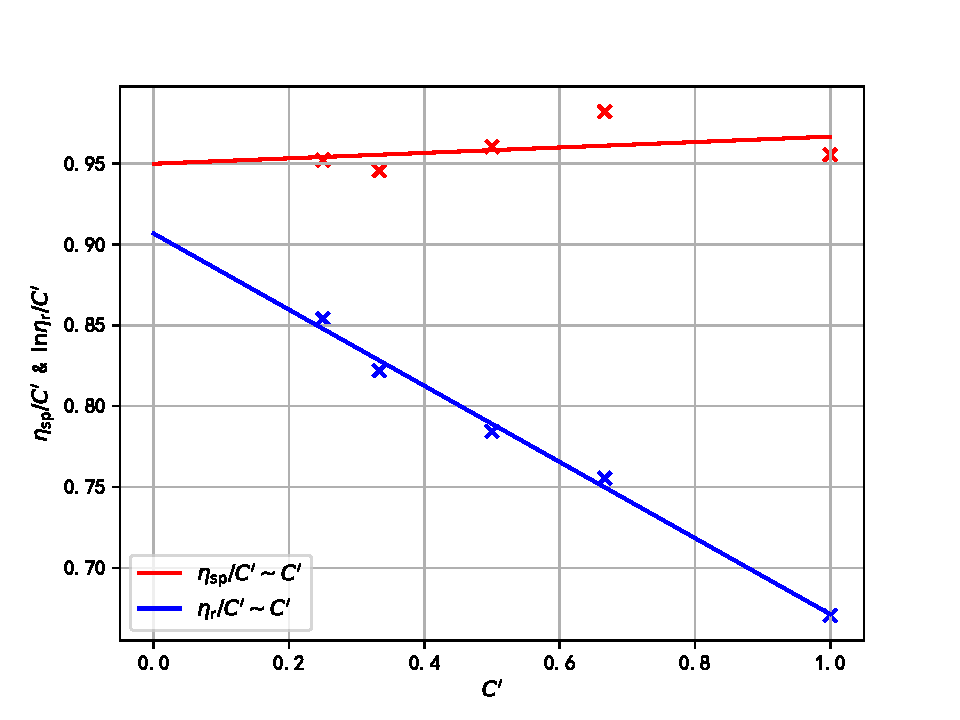
\includegraphics[scale=0.8]{fitting3.pdf}
    \caption{外推法法拟合曲线}
\end{figure}

拟合方程分别为
\begin{align}
    \frac{\eta_\text{sp}}{C'} &= 0.01677 C' + 0.9499, \\
    \frac{\ln\eta_\text{sp}}{C'} &= -0.2353 C' + 0.9067.
\end{align}

计算可得聚合物的特性粘数分别为52.77 mL/g、50.37 mL/g;粘均分子量
分别为$4.447\times 10^{4}$g/mol、$4.189\times 10^{4}$g/mol。
其分别对应 Huggins 方程和 Kraemer 方程得到的结果。

\subsection{误差分析}
\subsubsection{系统误差}

(1)数据处理所用方程的误差:Huggins 方程$\eta_{\text{sp}}/C'\sim C'$
和 Kraemer 方程$\ln\eta_\text{r}/C'\sim C'$是从基本方程
$\eta_\text{sp}/C = [\eta]/(1-k[\eta]C)$做级数展开后,分别保留
一阶项和二阶项得到的。前者适用于稀溶液,后者还必须要求$k = 1/3$,
否则图形将不是直线。因此方程本身在计算上存在一定的偏差,从而引入了
系统误差。

(2)数据处理时,使用溶液流出的时间之比近似代替粘度比,这种近似本身
就存在一定误差,因为溶液必须稀到一定程度才能满足这个近似条件。

(3)由于温度的传递具有滞后性,虽然使用了电动搅拌器,但仍不能保证
浴缸内各处温度完全均匀,并且温度计读数也具有滞后性,再加上测量液体
温度时并未将温度计直接与液体接触,由于玻璃的导热性也使得测量温度与
乌氏粘度计中的温度有一定的偏差。

\subsubsection{偶然误差}

(1)仪器固定粘度计的夹子较为松动,导致乌氏粘度计的毛细管部分难以
保持竖直,此外,由于搅拌装置的存在,而乌氏粘度计较轻,在搅拌装置的
作用下乌氏粘度计存在一定幅度的晃动,也无法保证在实验过程中完全竖直。

(2)由于高分子特性粘数与温度有一定关系,故该实验要求溶液恒温。查阅
资料得知,高聚物溶液粘度的测定对测试温度特别敏感,特性粘数随温度
升高而下降。一般而言,温度上升0.01$^\circ$C 粘度不受影响,温度上升
0.02$^\circ$C 特性粘数下降0.004,温度上升0.05$^\circ$C 特性粘数
下降0.011。但在实验中观察到恒温水浴的温度存在一定波动,有时能够存在
0.05$^\circ$C 左右的波动,温度的微小波动会导致实验结果的偏差。

(3)玻璃管壁会对溶液中的高分子有一定程度的吸附作用,这使得毛细管内
会形成一层薄聚乙二醇吸附层。吸附层的存在使得改变溶液浓度后的润洗效果
下降。若润洗不够完全,会使毛细管内溶液的浓度与实验设定的浓度有差异,
从而带来实验误差。

(4)科学界公认的人类极限反应时间为100 ms,即0.1 s;而对于未经训练
的普通人而言,反应时间通常在180 ms 左右。实验中需要按两次秒表,则
反应时间相差最高可达360 ms。同时,判断凹液面是否刚好经过刻度线时
会有主观影响,并且由于水浴缸中液体不断搅拌,光线的传播会有些许的
弯曲,液面是否刚好经过刻度线更加难以判断。这些原因都会导致测量时间
偶然误差的增大。

(6)实验中要求粘度计和待测液体洁净,虽然使用的液体均经过熔砂漏斗
过滤,但粘度计仍与大气相连通,空气中的粉尘仍可能进入粘度计中。尤其
是在吹气混合溶液时,吹入的气体并未经过无尘处理,空气中含有的粉尘
会直接进入粘度计中,影响最终溶液流出时间的测量准确性。

(7)用移液管向粘度计内加入液体时,移液管尖与液面有一段距离。这使得
加入的液体溅起较多水花,部分溶液溅至容器壁上,使粘度计内溶液的浓度
发生变化,带来误差。同时,在向粘度计内吹气混合溶液时,若吹气过猛,
则管内溶液会剧烈翻滚,部分溶液会溅至容器壁上无法流下,影响溶液的
浓度,最终给实验结果带来较大影响。

\subsection{实验讨论与改进方法}
\subsubsection{实验结果讨论}

本实验报告将实验法测得的结果作为最终的结果。因为由于测定时间时存在
一定的误差,使用外推法得到纯溶剂的流出时间会让这种误差得到成倍的
放大。因此使用外推法计算并不合理,实验法得到的结果更为准确。并且
由于 Huggins 方程只用了一次近似,而 Kraemer 方程用了两次近似,故
Huggins 方程的精确度更高。综上所述,聚乙二醇的粘均分子量为 3.316
$\times 10^4$ g/mol。

\subsubsection{实验原理改进}

本实验使用的方程是通过级数展开后近似得到的,因此可以通过增加展开的
次数以减小误差,以$\ln\eta_\text{r}/C'\sim C'$的 Kraemer 方程
为例,可以保留更高阶近似为
\begin{align}
    \frac{\ln\eta_\text{sp}}{C'}
    = [\eta] - \left(\frac{1}{2} - k\right)[\eta]^2 C'
    + \left(\frac{1}{3} - k\right)[\eta]^3 C'^2
    + \mathcal{O}(C'^4).
\end{align}

用此式进行非线性拟合,理论上可以得到更加精确的结果。

\subsubsection{实验方法改进}

秦建彬等人$^{[2]}$用 GPC 法测定聚合物平均分子量的实验。该实验操作
相对简单。实验的关键在于选用与 GPC 流动相相同的溶剂。配置好的溶液
经过微孔滤膜过滤后再注入色谱柱,设置好仪器参数,整个测试过程由 GPC
快速且自动的完成。实验的可操作性与实验结果数据明显优于使用乌氏黏度计
测定聚合物平均分子量。

\section{结语}

用稀溶液粘度法可以测量有机高分子的相对分子质量,用实验法和外推法、
$\eta_{\text{sp}}/C'\sim C'$的 Huggins 方程和
$\ln\eta_\text{r}/C'\sim C'$的 Kraemer 方程都可以得到纯溶剂的
流动时间。实验测得的相对分子质量为3.316$\times 10^4$ g/mol。
本实验由于外界影响大,实验操作引起的误差较大,整体实验测量精度较差。
若使用更精准的仪器、使用更精确的处理方法,可以得到更精确的相对分子
质量。

\begin{center}
    \Large\bfseries{参考文献}
\end{center}
\noindent
[1] 傅献彩, 沈文霞, 姚天扬等. 物理化学(第五版). 上册[M].
高等教育出版社,2006.

\noindent
[2] 秦建彬, 史学涛, 李春梅, 狄西岩, 张广成, 焦剑. 关于乌氏黏度计法
与凝胶渗透色谱法测定聚合物平均分子量实验的讨论[J]. 化工高等教育,
2020, 37(02): 151-154.


\newpage

\begin{center}
    \LARGE\bfseries{附录~~~实验数据处理}
\end{center}
\begin{center}
    \Large\bfseries{附录I~~~实验数据处理}
\end{center}

\subsection*{I.1~~~实验法数据处理}

当溶液浓度很低时,$\rho\approx\rho_0$,故有
\begin{align}
    \eta_\text{r} &= \frac{\eta}{\eta_0}
    \approx \frac{t}{t_0},
    \tag{I.1} \\
    \eta_\text{sp} &= \eta_\text{r} - 1
    \approx \frac{t}{t_0} - 1.
    \tag{I.2}
\end{align}

由此近似可得下表
\begin{longtable}{ccccccc}
    \caption{实验数据计算(一)} \\
    \hline
    溶剂量/mL & 相对浓度$C'$ & 平均流出时间$t$/s & 相对粘度$\eta_\text{r}$ & 特性粘度$\eta_{\text{sp}}$ & $\eta_\text{sp}/C'$ & $\ln\eta_\text{r}/C'$ \\
    \hline
    $0$  & $ 1 $ & $3'36''37$ & $1.8836$ & $0.8836$ & $0.8836$ & $0.6332$ \\
    $5$  & $2/3$ & $3'03''19$ & $1.5941$ & $0.5941$ & $0.8912$ & $0.6995$ \\
    $5$  & $1/2$ & $2'43''59$ & $1.4259$ & $0.4259$ & $0.8518$ & $0.7096$ \\
    $10$ & $1/3$ & $2'25''42$ & $1.2670$ & $0.2670$ & $0.8010$ & $0.7100$ \\
    $10$ & $1/4$ & $2'17''09$ & $1.1926$ & $0.1926$ & $0.7704$ & $0.7045$ \\
    纯溶剂 & $0$ & $1'55''00$ & $1.0000$ & $0.0000$ & / & / \\
    \hline
\end{longtable}

由 Huggins 方程
\begin{align}
    \frac{\eta_\text{sp}}{C} = [\eta] + k[\eta]^2 C
    \tag{I.3}
\end{align}
和 Kraemer 方程
\begin{align}
    \frac{\ln\eta_\text{r}}{C} = [\eta] - \beta[\eta]^2 C,
    \tag{I.4}
\end{align}
以$\eta_\text{sp}/C'$和$\ln\eta_\text{r}/C'$分别对$C'$作图,即
\begin{align}
    \frac{\eta_\text{sp}}{C'}
        = [\eta]C_0 + k[\eta]^2 C_0^2 C',
    \tag{I.5} \\
    \frac{\ln\eta_\text{r}}{C'}
        = [\eta]C_0 - \beta[\eta]^2 C_0^2 C'.
    \tag{I.6}
\end{align}
得到的结果如图 4.4 所示。

\begin{figure}[!h]
    \centering
    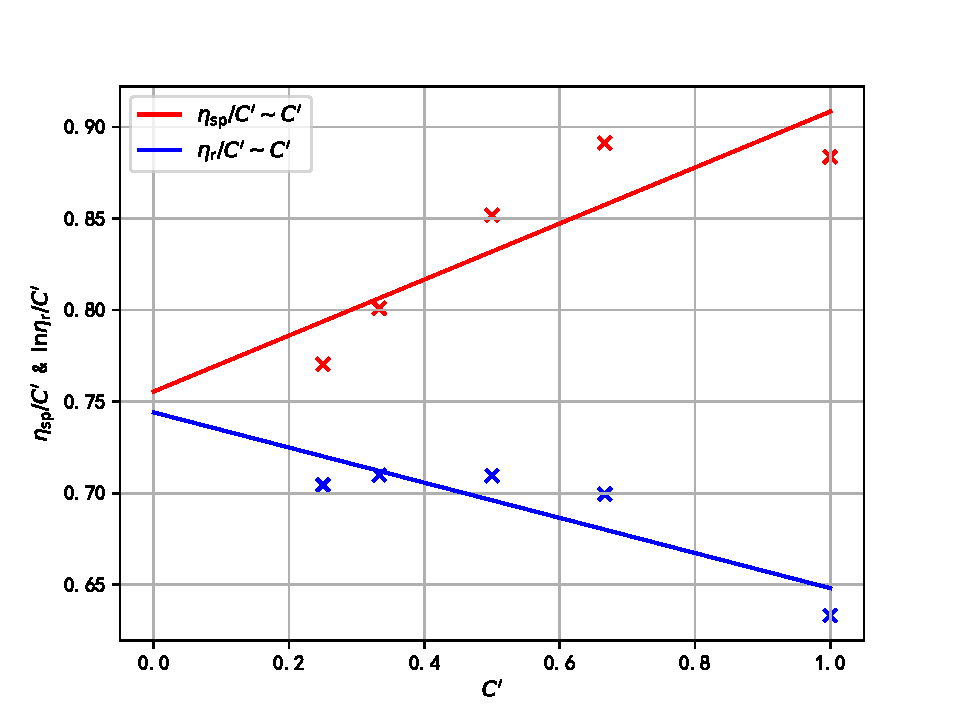
\includegraphics[scale=0.8]{fitting1.pdf}
    \caption{直接作图法拟合曲线}
\end{figure}

拟合方程为
\begin{align}
    \frac{\eta_\text{sp}}{C'} &= 0.1528 C' + 0.7555,
    \tag{I.7} \\
    \frac{\ln\eta_\text{r}}{C'} &= -0.09595 C' + 0.7441.
    \tag{I.8}
\end{align}

对比实验原理中的方程可知,直线的截距即为$[\eta]C_0$。对于 Huggins
方程,截距为$[\eta]C_0 = 0.7555$。溶液初始浓度$C_0$为$0.018$
g/mL,故可得$[\eta] = 41.97$mL/g。

由
\begin{align}
    [\eta] = KM^a, \tag{I.9}
\end{align}
查表可知,对于聚乙二醇,$a = 0.78$,$K = 0.0125$mL/g。故聚合物的
粘均分子量为
\begin{align}
    \overline{M}_\eta
    &= \left(\frac{[\eta]}{K}\right)^{1/a} \notag\\
    &= \left(\frac{41.97}{0.0125}\right)^{1/0.78}
        \tag{I.10}\\
    &= 3.316\times 10^{4}~\mathrm{(g/mol)}. \notag
\end{align}

同理,对于 Kraemer 方程,可得$[\eta] = 41.34$mL/g,粘均分子量为
$3.252\times 10^{4}~\mathrm{g/mol}$。

\subsection*{I.2~~~外推法数据处理}

由除纯溶剂外的实验数据可作出$t\sim C'$图如图 4.5 所示。
\begin{figure}[!h]
    \centering
    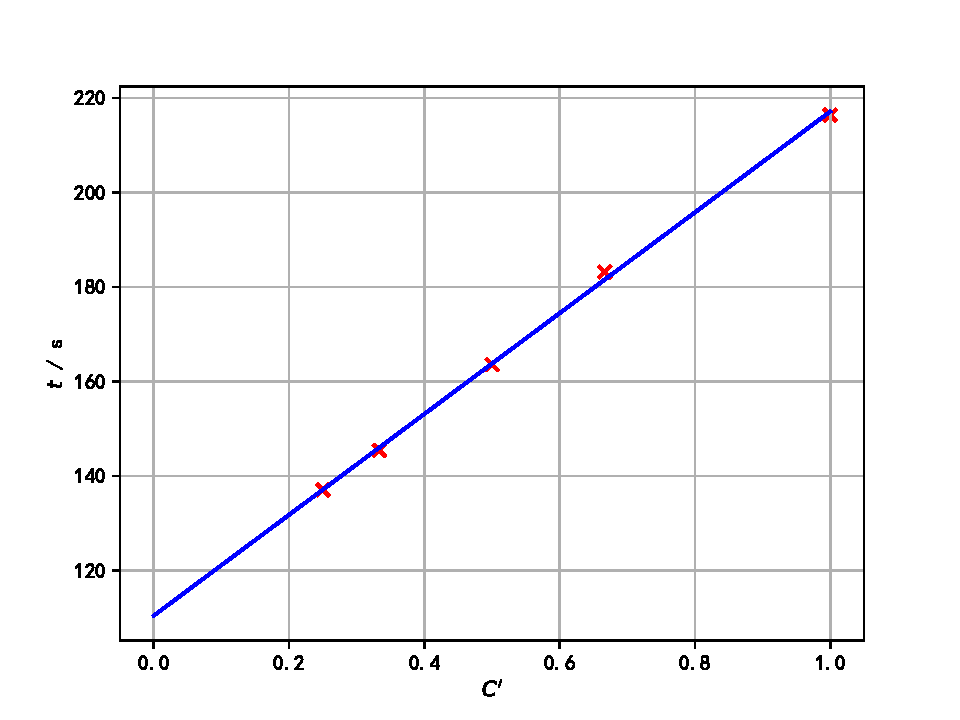
\includegraphics[scale=0.8]{fitting2.pdf}
    \caption{$t\sim C'$拟合直线}
\end{figure}

拟合方程为
\begin{align}
    t = 106.63 C' +110.47
    \tag{I.11}
\end{align}

其截距可视为纯溶剂的流出时间,为110.47 s。

由近似式(I.1)、(I.2)可得数据计算表格如下
\begin{longtable}{ccccccc}
    \caption{实验数据计算(二)} \\
    \hline
    溶剂量/mL & 相对浓度$C'$ & 平均流出时间$t$/s & 相对粘度$\eta_\text{r}$ & 特性粘度$\eta_{\text{sp}}$ & $\eta_\text{sp}/C'$ & $\ln\eta_\text{r}/C'$ \\
    \hline
    $0$  & $ 1 $ & $3'36''37$ & $1.9553$ & $0.9553$ & $0.9553$ & $0.6705$ \\
    $5$  & $2/3$ & $3'03''19$ & $1.6547$ & $0.6547$ & $0.9821$ & $0.7554$ \\
    $5$  & $1/2$ & $2'43''59$ & $1.4802$ & $0.4802$ & $0.9604$ & $0.7844$ \\
    $10$ & $1/3$ & $2'25''42$ & $1.3152$ & $0.3152$ & $0.9456$ & $0.8220$ \\
    $10$ & $1/4$ & $2'17''09$ & $1.2380$ & $0.2380$ & $0.9520$ & $0.8540$ \\
    纯溶剂 & $0$ & $1'50''47$ & $1.0000$ & $0.0000$ & / & / \\
    \hline
\end{longtable}

拟合图像如图 4.6 所示。
\begin{figure}[!h]
    \centering
    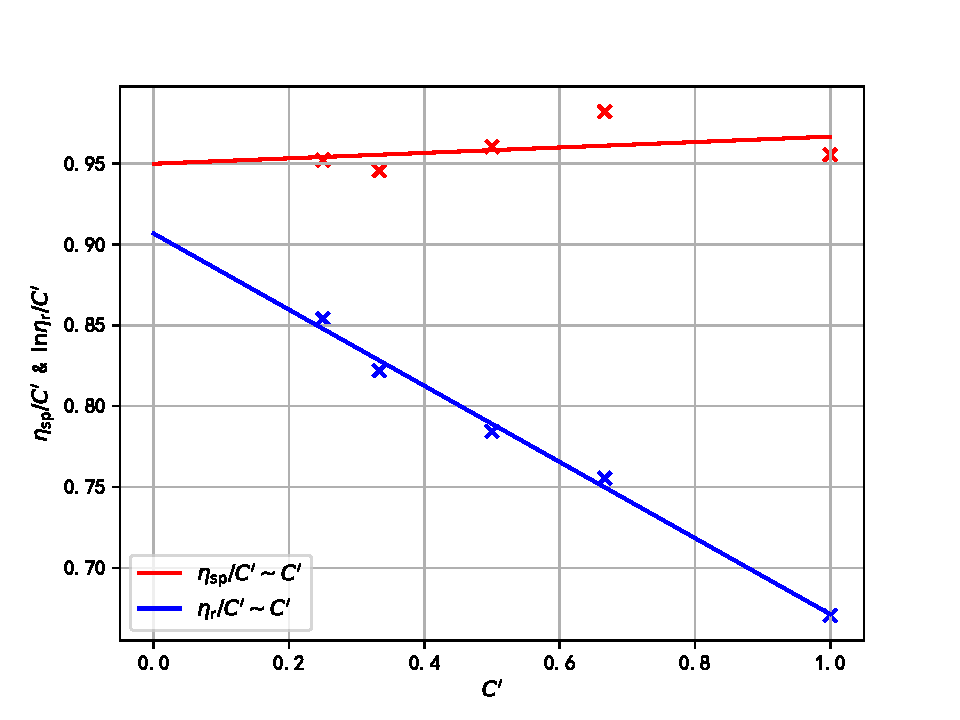
\includegraphics[scale=0.8]{fitting3.pdf}
    \caption{外推法法拟合曲线}
\end{figure}

拟合方程为
\begin{align}
    \frac{\eta_\text{sp}}{C'} &= 0.01677 C' + 0.9499,
    \tag{I.12} \\
    \frac{\ln\eta_\text{sp}}{C'} &= -0.2353 C' + 0.9067.
    \tag{I.13}
\end{align}

用与 I.1 节同样的方法计算可得聚合物的特性粘数分别为52.77 mL/g、
50.37 mL/g;粘均分子量分别为$4.447\times 10^{4}$g/mol、
$4.189\times 10^{4}$g/mol。其分别对应 Huggins 方程和 Kraemer
方程得到的结果。

\newpage
\begin{center}
    \Large\bfseries{附录II~~~原始数据记录}
\end{center}

浓溶液密度:0.9989 g/mL;稀溶液密度:0.9966 g/mL;水的密度:
0.9957 g/mL。

粘度计编号:98号;毛细管内径$r = 0.55$mm;称取聚乙二醇质量:
1.0001 g。

\begin{longtable}{cccccc}
    \caption{实验原始数据} \\
    \hline
    加入溶剂体积/mL & 相对浓度 & \multicolumn{3}{c}{流出时间} & 平均值/s \\
    \hline
    $0 $ & $ 1 $ & $3'46''40$ & $3'36''33$ & $3'36''37$ & $3'36''37$ \\
    $5 $ & $2/3$ & $3'02''97$ & $3'03''13$ & $3'03''46$ & $3'03''19$ \\
    $5 $ & $1/2$ & $2'43''37$ & $2'44''06$ & $2'43''34$ & $2'43''59$ \\
    $10$ & $1/3$ & $2'25''47$ & $2'25''43$ & $2'25''37$ & $2'25''42$ \\
    $10$ & $1/4$ & $2'17''09$ & $2'17''09$ & $2'17''09$ & $2'17''09$ \\
    \hline
    \multicolumn{2}{c}{纯溶剂流出时间/s}
                 & $1'55''09$ & $1'54''93$ & $1'54''97$ & $1'55''00$ \\
    \hline
\end{longtable}

\end{document}


